\subsection{Section 3.3}

\begin{tcolorbox}[
        title={Problem 24},
        valign=center,
        nobeforeafter,
        colframe=gray!95!black
    ]
Let \(f(x, y) = Ax^2 + B\), where \(A\) and \(B\) are constants. \\

What are the critical points of \(f\)? Are they local maxima or local minima?
\end{tcolorbox}

\begin{solution}
    We first compute the gradient of \(f\):
    \begin{align}
        \nabla f(x, y) &= \left(2Ax, 0\right)
    \end{align}
    
    The gradient is equal to \((0, 0)\) when \((x, y) = (0, y)\) where \(y\) is allowed to vary.
    
    The critical points of \(f\) are all the points along the \(y\)-axis.
    
    Recall one definition of local extrema:
    \begin{itemize}
        \item \((x_0, y_0)\) is a local minimum if the Hessian \(H_f(x_0, y_0)\) is positive semidefinite.
        \item \((x_0, y_0)\) is a local maximum if the Hessian \(H_f(x_0, y_0)\) is negative semidefinite.
    \end{itemize}
    
    Recall also the definition of positive and negative semidefinite:
    \begin{itemize}
        \item A \(2 \times 2\) or \(3 \times 3\) matrix \(A\) is positive definite if \(a_{11} > 0\) and \(\det(A) > 0\)
        \item A \(2 \times 2\) or \(3 \times 3\) matrix \(A\) is negative definite if \(a_{11} < 0\) and \(\det(A) < 0\)
    \end{itemize}
    
    We now compute the Hessian matrix of \(f\):
    \begin{align*}
        H_f(0, y) &= 
        \begin{pmatrix}
            \frac{\partial^2 f}{\partial x^2} & \frac{\partial^2 f}{\partial y \partial x} \\
            \frac{\partial^2 f}{\partial x \partial y} & \frac{\partial^2 f}{\partial y^2} 
        \end{pmatrix} \\
        &= 
        \begin{pmatrix}
            \frac{\partial}{\partial x}(2Ax) & \frac{\partial}{\partial y}(2Ax) \\
            \frac{\partial}{\partial x}(0) & \frac{\partial}{\partial y}(0)
        \end{pmatrix} \\
        &= 
        \begin{pmatrix}
            2A & 0 \\
            0 & 0
        \end{pmatrix}
    \end{align*}
    
    We now compute the determinant:
    \begin{align}
        \det\left(H_f(0, y)\right) &= 2A(0) - 0 \\
        &= 0
    \end{align}
    
    Unfortunately we cannot gather any information since \(\det\left(H_f(0, y)\right) = 0\). We therefore proceed by inspection.
    
    Observe that \(f(x, y)\) does not actually depend on \(y\). We fix some arbitrary \(y = y_0\). Then \(f(x, y) = f(x)\).
    
    From single variable calculus, the concavity of a function \(f\) is determined by the second derivative of \(f\):
    \begin{align*}
        f''(x) &= (Ax^2 + B)'' \\
        &= (2Ax)' \\
        &= 2A
    \end{align*}
    
    Then \(x = 0\) is a local minimum if \(A > 0\) and \(x = 0\) is a local maximum if \(A < 0\).
    
    Similarly, \((x, y) = (0, y)\) are local minima if \(A > 0\) and \((0, y) = (0, y)\) are local maxima if \(A < 0\).
\end{solution}

\begin{tcolorbox}[
        title={Problem 44},
        valign=center,
        nobeforeafter,
        colframe=gray!95!black
    ]
Let \(f(x, y) = 1 + xy + x - 2y\) and let \(D\) be the triangular region in \(\mathbb{R}^2\) with vertices \((1, -2)\), \((5, -2)\), and \((1, 2)\). \\

Find the absolute maximum and minimum values of \(f\) on \(D\). Give all points where these extreme values occur.
\end{tcolorbox}

\begin{solution}
    We first compute the gradient of \(f\):
    \begin{align}
        \nabla f(x, y) &= \left(y + 1, x - 2\right)
    \end{align}
    
    The gradient is equal to \((0, 0)\) when \((x, y) = (2, -1)\).
    
    The only critical point of \(f\) in \(D\) is \((x, y) = (2, -1)\).
    
    We now proceed to find all extrema of \(f\) on the boundary.
    
    \begin{figure}[h]
        \centering
        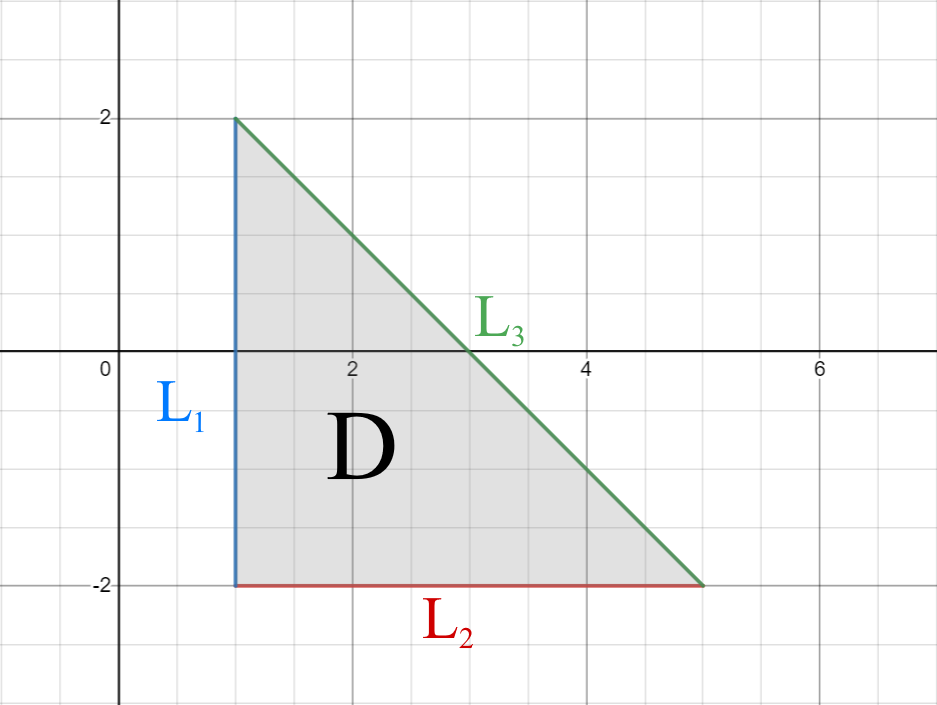
\includegraphics[width=0.4\textwidth]{Pictures/Tutorial 3-1.png}
        \caption{Triangular region in \(\mathbb{R}^2\) with vertices \((1, -2)\), \((5, -2)\), and \((1, 2)\).}
    \end{figure}
    
    On the curve \(L_1\), we have \(x = 1\) and \(-2 \leq y \leq 2\). 
    
    Then:
    \begin{align*}
        f(1, y) &= 1 + y + 1 - 2y \\
        &= 2 - y
    \end{align*}
    
    Since this function is linear, the extrema are at the endpoints: \((x, y) = (1, -2)\) and \((x, y) = (1, 2)\).
    
    On the curve \(L_2\), we have \(y = -2\) and \(1 \leq x \leq 5\). 
    
    Then:
    \begin{align*}
        f(x, -2) &= 1 -2x + x + 4 \\
        &= 5 - x
    \end{align*}
    
    Since this function is linear, the extrema are at the endpoints: \((x, y) = (1, -2)\) and \((x, y) = (5, -2)\).
    
    To find the extrema on the curve \(L_3\), we must solve for \(y\) in terms of \(x\).
    
    Observe that the curve is linear. Then \(y = mx + b\).
    
    Since we are given two points on the curve, \((x, y) = (1, 2)\) and \((x, y) = (5, -2)\), we can find the slope:
    \begin{align*}
        m &= \frac{-2 - 2}{5 - 1} \\
        &= -1
    \end{align*}
    
    Then \(y = -x + b\).
    
    To find the \(y\)-intercept, we plug in \((x, y) = (1, 2)\):
    \begin{align*}
        y &= -x + b \\
        2 &= -1 + b \\
        3 &= b
    \end{align*}
    
    Then we have that \(L_3\) is given by the function \(y = -x + 3\).
    
    Then:
    \begin{align*}
        f(x, -x + 3) &= 1 + x(-x + 3) + x - 2(-x + 3) \\
        &= 1 - x^2 + 3x + x + 2x - 6 \\
        &= - x^2 + 6x - 5
    \end{align*}
    
    From single variable calculus, we find the extrema of \(f\) on \(L_3\) by taking the derivative of \(f\):
    \begin{align*}
        f'(x, -x + 3) &= -2x + 6
    \end{align*}
    
    The derivative is equal to zero when \(x = 3\). This implies that \(y = 0\).
    
    Our points of interest are therefore \((2, -1)\), \((1, -2)\), \((1, 2)\), \((5, -2)\), and \((3, 0)\).
    
    The values of \(f\) at these points are given by:
    \begin{align*}
        f(2, -1) &= 3 & f(1, -2) &= 4 \\
        f(1, 2) &= 0 & f(5, -2) &= 0 \\
        f(3, 0) &= 4
    \end{align*}
    
    By observation, \(f(1, -2) = f(3, 0) = 4\) are maxima and \(f(1, 2) = f(5, -2) = 0\) are minima.
\end{solution}

\subsection{Section 3.4}

\begin{tcolorbox}[
        title={Problem 2},
        valign=center,
        nobeforeafter,
        colframe=gray!95!black
    ]
Consider all rectangles with fixed perimeter \(p\). \\

Use Lagrange multipliers to show that the rectangle with maximal area is a square.
\end{tcolorbox}

\begin{proof}
Let \(x\) be the width and \(y\) be the height of the rectangle.

Then the area \(A\) and perimeter \(p\) are given by:
\begin{align}
    A &= xy & p = 2x + 2y
\end{align}

We wish to maximize \(f(x, y) = A\) subject to the constraint \(g(x, y) = 2x + 2y - p = 0\).

We compute the gradients of \(f\) and \(g\):
\begin{align}
    \nabla f(x, y) &= \left(y, x\right) & \nabla g(x, y) &= \left(2, 2\right) 
\end{align}

By the Lagrange Multiplier Theorem:
\begin{align}
    \nabla f &= \lambda \nabla g \\
    \left(y, x\right) &= \lambda \left(2, 2\right) \\
    \left(y, x\right) &= \left(2\lambda, 2\lambda\right)
\end{align}

We must now solve the following set of equations:
\begin{align}
    \begin{cases}
        y &= 2\lambda \\
        x &= 2\lambda
    \end{cases}
\end{align}

By observation, we find that the \(x = y\). The rectangle with maximal area is therefore a square.
\end{proof}

\begin{tcolorbox}[
        title={Problem 6},
        valign=center,
        nobeforeafter,
        colframe=gray!95!black
    ]
Let \(f(x, y, z) = x + y + z\) be subject to constraints \(x^2 - y^2 = 1\) and \(2x + z = 1\). \\

Find the extrema of \(f\) subject to the stated constraints.
\end{tcolorbox}

\begin{solution}
    Let \(g(x, y, z) = x^2 - y^2 - 1 = 0\) and \(h(x, y, z) = 2x + z - 1\). 
    
    We first compute the gradients of \(f\), \(g\), and \(h\):
    \begin{align}
        \nabla f(x, y, z) &= (1, 1, 1) & \nabla g(x, y, z) &= (2x, -2y, 0) & \nabla h(x, y, z) &= (2, 0, 1) 
    \end{align}
    
    By the Lagrange Multiplier Theorem:
    \begin{align}
        \nabla f &= \lambda \nabla g + \mu \nabla h \\
        (1, 1, 1) &= \lambda (2x, -2y, 0) + \mu (2, 0, 1) \\
        (1, 1, 1) &= (2\lambda x, -2\lambda y, 0) + (2\mu, 0, \mu) \\
        (1, 1, 1) &= (2\lambda x + 2\mu, -2\lambda y, \mu)
    \end{align}
    
    We must now solve the following set of equations:
    \begin{align}
        \begin{cases}
            1 &= 2\lambda x + 2\mu \\
            1 &= -2\lambda y \\
            1 &= \mu
        \end{cases}
        &=
        \begin{cases}
            1 &= 2\lambda x + 2 \\
            1 &= -2\lambda y
        \end{cases} \\
        &=
        \begin{cases}
            -1 &= 2\lambda x \\
            1 &= -2\lambda y
        \end{cases} \\
        &=
        \begin{cases}
            -\frac{1}{2\lambda} &= x \\
            -\frac{1}{2\lambda} &= y
        \end{cases}
    \end{align}
    
    By observation, we find that \(x = y\). This is impossible since we contradict our constraint \(x^2 - y^2 = 1\):
    \begin{align*}
        x^2 - y^2 &= \left(-\frac{1}{2\lambda}\right)^2 - \left(-\frac{1}{2\lambda}\right)^2 \\
        &= 0 \\
        &\neq 1
    \end{align*}
    
    This is a contradiction. Therefore, there are no extrema of \(f\) subject to these constraints.
\end{solution}

\begin{claim}
    \textbf{(For those who wish to understand why)} There are no extrema of \(f\) subject to these constraints because \(f(x, y, z)\) is monotonically increasing along these constraints.
\end{claim}

\begin{proof}
    We manipulate the constraints:
    \begin{align*}
        x^2 - y^2 &= 1 & 2x + z &= 1 \\
        x^2 &= y^2 + 1 & z &= 1 - 2x \\
        x &= \pm \sqrt{y^2 + 1} & z &= 1 - 2\left(\pm \sqrt{y^2 + 1}\right) \\
        & & z &= 1 \mp 2\sqrt{y^2 + 1}
    \end{align*}
    
    Observe that we may write \(x\) and \(z\) as a function of \(y\). 
    
    The function \(f(x, y, z)\) along these constraints can then be written as a single variable function:
    \begin{align*}
        f(x(y), y, z(y)) &= x(y) + y + z(y) \\
        &= \pm \sqrt{y^2 + 1} + y + 1 \mp 2\sqrt{y^2 + 1} \\
        &= \pm \sqrt{y^2 + 1} + y + 1 \mp 2\sqrt{y^2 + 1} \\
        &= \mp \sqrt{y^2 + 1} + y + 1
    \end{align*}
    
    The two solutions are:
    \begin{align}
        f_1(y) &= \sqrt{y^2 + 1} + y + 1 & f_2(y) &= -\sqrt{y^2 + 1} + y + 1
    \end{align}
    
    We compute the derivatives of \(f_1\) and \(f_2\):
    \begin{align}
        f'_1(y) &= \frac{y}{\sqrt{y^2 + 1}} + 1 & f'_2(y) &= -\frac{y}{\sqrt{y^2 + 1}} + 1
    \end{align}
    
    Observe that for all \(y \in \mathbb{R}\):
    \begin{align}
        \frac{y}{\sqrt{y^2 + 1}} &\geq -1 & -\frac{y}{\sqrt{y^2 + 1}} &\geq -1
    \end{align}
    
    A function \(f(x)\) is monotonically increasing if \(f'(x) \geq 0\) for all \(x \in \mathbb{R}\).
    
    Observe that:
    \begin{align}
        f'_1(y) &= \frac{y}{\sqrt{y^2 + 1}} + 1 & f'_2(y) &= -\frac{y}{\sqrt{y^2 + 1}} + 1 \\
        &\geq -1 + 1 & &\geq -1 + 1 \\
        &= 0 & &= 0
    \end{align}
    
    Then \(f_1\) and \(f_2\) are monotonically increasing and therefore have no extrema. This is similar to how \(f(x) = x\) has no extrema.
\end{proof}

\begin{tcolorbox}[
        title={Problem 6 (Modified)},
        valign=center,
        nobeforeafter,
        colframe=gray!95!black
    ]
    
The problem was modified to provide students with a non-trivial solution using Lagrange Multipliers. \\

Let \(f(x, y, z) = x + y + z\) be subject to constraints \(x^2 + y^2 = 1\) and \(2x + z = 1\). \\

Find the extrema of \(f\) subject to the stated constraints.
\end{tcolorbox}

\begin{solution}
    Let \(g(x, y, z) = x^2 + y^2 - 1 = 0\) and \(h(x, y, z) = 2x + z - 1\). 
    
    We first compute the gradients of \(f\), \(g\), and \(h\):
    \begin{align}
        \nabla f(x, y, z) &= (1, 1, 1) & \nabla g(x, y, z) &= (2x, 2y, 0) & \nabla h(x, y, z) &= (2, 0, 1) 
    \end{align}
    
    By the Lagrange Multiplier Theorem:
    \begin{align}
        \nabla f &= \lambda \nabla g + \mu \nabla h \\
        (1, 1, 1) &= \lambda (2x, 2y, 0) + \mu (2, 0, 1) \\
        (1, 1, 1) &= (2\lambda x, 2\lambda y, 0) + (2\mu, 0, \mu) \\
        (1, 1, 1) &= (2\lambda x + 2\mu, 2\lambda y, \mu)
    \end{align}
    
    We must now solve the following set of equations:
    \begin{align}
        \begin{cases}
            1 &= 2\lambda x + 2\mu \\
            1 &= 2\lambda y \\
            1 &= \mu
        \end{cases}
        &=
        \begin{cases}
            1 &= 2\lambda x + 2 \\
            1 &= 2\lambda y
        \end{cases} \\
        &=
        \begin{cases}
            -1 &= 2\lambda x \\
            1 &= 2\lambda y
        \end{cases} \\
        &=
        \begin{cases}
            -\frac{1}{2\lambda} &= x \\
            \frac{1}{2\lambda} &= y
        \end{cases}
    \end{align}
    
    Since we have found \(x\) and \(y\) in terms of \(\lambda\), we substitute \(x\) and \(y\) from the first constraint:
    \begin{align*}
        x^2 + y^2 &= 1 \\
        \left(-\frac{1}{2\lambda}\right)^2 + \left(\frac{1}{2\lambda}\right)^2 &= 1 \\
        \frac{1}{4\lambda^2} + \frac{1}{4\lambda^2} &= 1 \\
        \frac{2}{4\lambda^2} &= 1 \\
        \frac{1}{2} &= \lambda^2 \\
        \pm\frac{1}{\sqrt{2}} &= \lambda
    \end{align*}
    
    We find that:
    \begin{align*}
        x &= -\frac{1}{2\lambda} & y &= \frac{1}{2\lambda} \\
        &= \mp \frac{\sqrt{2}}{2} & &= \pm \frac{\sqrt{2}}{2} \\
        &= \mp \frac{1}{\sqrt{2}} & &= \pm \frac{1}{\sqrt{2}}
    \end{align*}
    
    From the second constraint, we find that:
    \begin{align*}
        2x + z &= 1 \\
        z &= 1 - 2x \\
        z &= 1 - 2\left(\mp \frac{1}{\sqrt{2}}\right) \\
        z &= 1 \pm \sqrt{2} 
    \end{align*}

    The points of interest are therefore \((x, y, z) = \left(-\frac{1}{\sqrt{2}}, \frac{1}{\sqrt{2}}, 1 + \sqrt{2}\right)\) and \((x, y, z) = \left(\frac{1}{\sqrt{2}}, -\frac{1}{\sqrt{2}}, 1 - \sqrt{2}\right)\).
    
    We compute the values of \(f\) at these points:
    \begin{align*}
        f\left(-\frac{1}{\sqrt{2}}, \frac{1}{\sqrt{2}}, 1 + \sqrt{2}\right) &= -\frac{1}{\sqrt{2}} + \frac{1}{\sqrt{2}} + 1 + \sqrt{2} & f\left(\frac{1}{\sqrt{2}}, -\frac{1}{\sqrt{2}}, 1 - \sqrt{2}\right) &= \frac{1}{\sqrt{2}} - \frac{1}{\sqrt{2}} + 1 - \sqrt{2} \\
        &= 1 + \sqrt{2} & &= 1 - \sqrt{2}
    \end{align*}
    
    Then \(f\left(-\frac{1}{\sqrt{2}}, \frac{1}{\sqrt{2}}, 1 + \sqrt{2}\right) = 1 + \sqrt{2}\) is a maximum and \(f\left(\frac{1}{\sqrt{2}}, -\frac{1}{\sqrt{2}}, 1 - \sqrt{2}\right) = 1 - \sqrt{2}\) is a minimum.
\end{solution}